\documentclass[a4paper,12pt]{article}
\usepackage[utf8]{inputenc}
\usepackage[russian]{babel}
\usepackage{amsmath}
\usepackage{amssymb}
\usepackage{hyperref}
\usepackage{geometry}
\usepackage{graphicx}
\geometry{left=2.5cm,right=2.5cm,top=2cm,bottom=2cm}


\begin{document}

\fontsize{12}{17}\selectfont
\begin{center} 
   \Large ГУО "Белорусский государственный университет \par
   информатики и радиотехники"\par
   Факультет информационных технологий и управления\par
   Кафедра интеллектуальных информационных технологий
   \end{center} \setlength{\parskip}{8cm} \par

\begin{center}

 \Large Расчетная работа
 \par \setlength{\parskip}{0.5cm}
\Large «Графы. Решение теоретико-графовой задачи»
\end{center}
\setlength{\parskip}{5cm}
\begin{flushright}
    Подготовил: \par
 \setlength{\parskip}{0.2cm}   
Басак Ю. \par
Гр.421702 \par
Проверил: 

Малиновская Н. В.
\setlength{\parskip}{2cm}
\begin{center}

Минск 2024
\end{center}

\end{flushright}
\section*{Цель работы}
   \setlength{\parskip}{1cm}
\begin{itemize}
    \item Изучить теорию графов и смежных матриц
    \item Изучить алгоритм нахождения декартового произведения графов
    \item Реализовать алгоритм нахождения декартового произведения на языке программирования
    \item Уметь использовать основные алгоритмы при работе с графами
\end{itemize}

\section*{Условие задания}
Выполнить свой вариант расчетной работы и перенести получившееся решение на язык программирования C++

\section*{Вариант}
Для рассчетной работы мне был выдан вариант 4.1. Выполнить с помощью смежной матрицы


\section*{Теоретические сведения для выполнения расчетной работы}
\begin{itemize}
    \item \textbf{Граф}: набор вершин и ребер, соединяющих эти вершины.
    \item \textbf{Вершина}: один из объектов, соединенных ребрами в графе.
    \item \textbf{Ребро}: связь между двумя вершинами.
    \item \textbf{Неориентированный граф}: граф, в котором ребра не имеют направления.
    \item \textbf {Декартовое произведение графов}: способ объединения двух графов, создавая новый граф, в котором вершины представляют собой пары вершин из первого и второго графа и в котором между двумя вершинами существует ребро, если они соответствуют вершинам исходных графов, которые соединены определенным образом.
    
    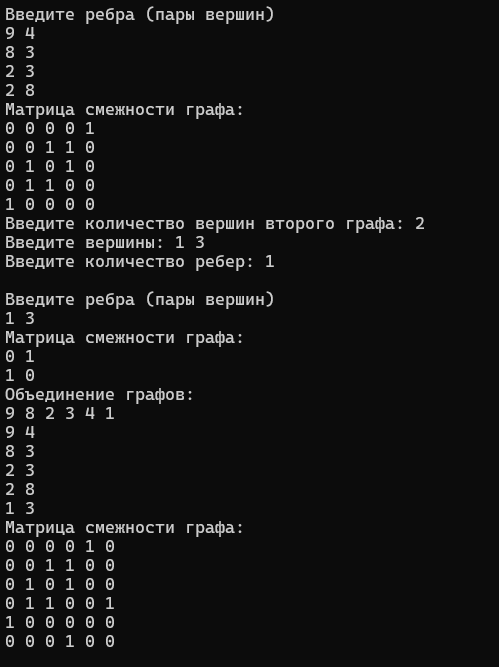
\includegraphics[width=0.9\columnwidth]{4.png}
    \item \textbf{Смежная матрица}: таблица, которая показывает, как вершины (узлы) графа соединены друг с другом.

    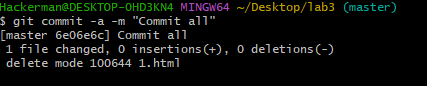
\includegraphics[width=0.9\columnwidth]{6.png}
    
\end{itemize}




\section*{Пример выполнения кода}
  \setlength{\parskip}{0.2cm}
\item \textbf{Первый пример}
  \setlength{\parskip}{0.2cm}

 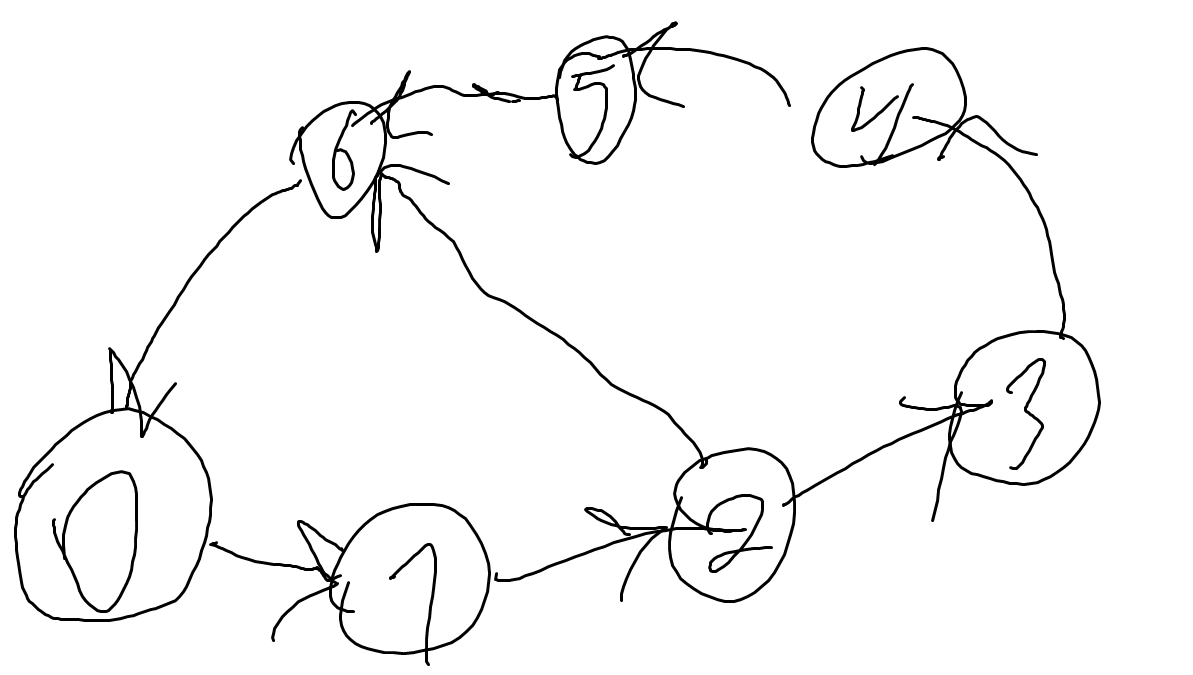
\includegraphics[width=0.9\columnwidth]{1.png}
 \item \textbf{Второй пример}
  \setlength{\parskip}{0.2cm}
  
 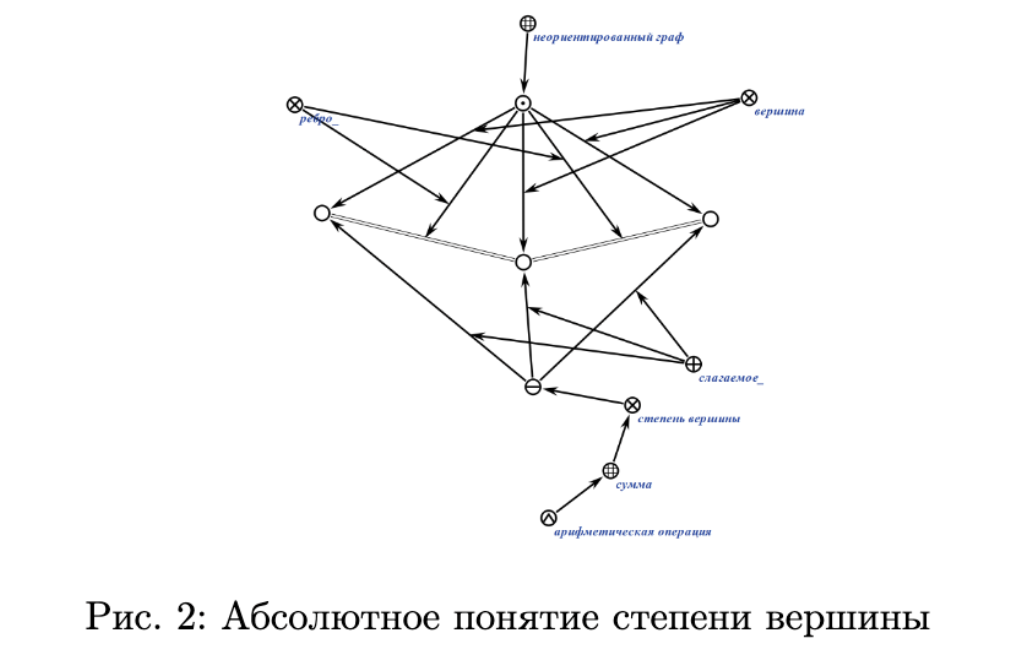
\includegraphics[width=0.9\columnwidth]{2.png}
  \item \textbf{Третий пример}
  \setlength{\parskip}{0.2cm}
  
 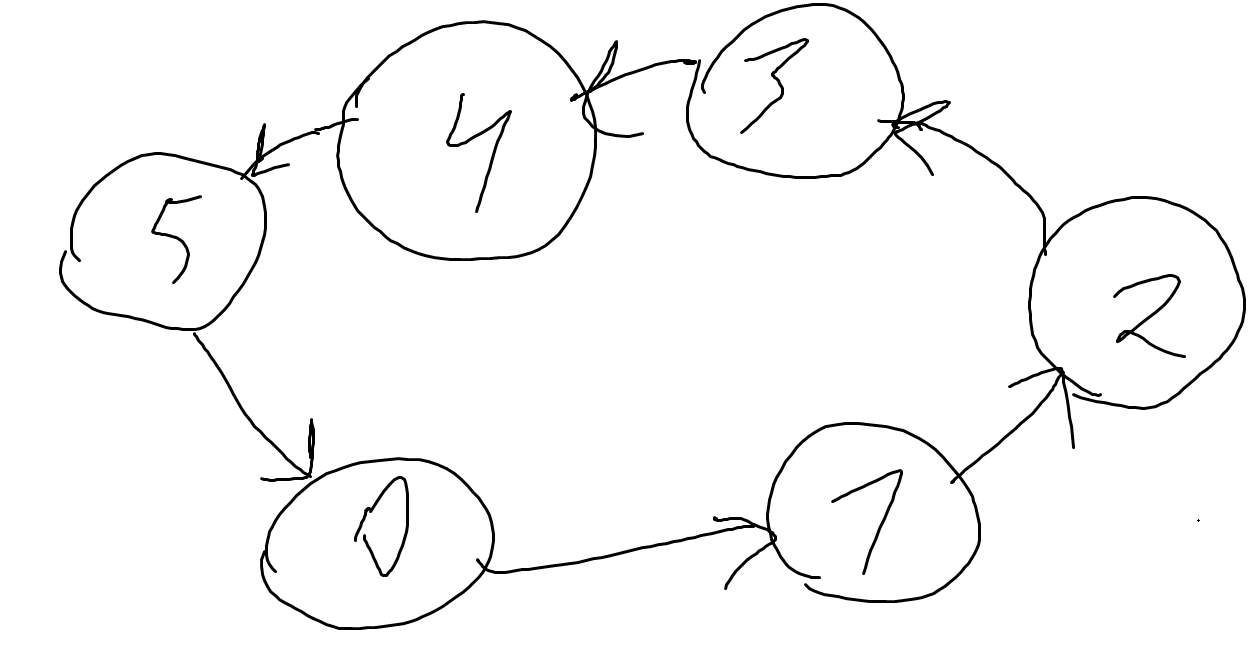
\includegraphics[width=0.9\columnwidth]{3.png}
\section*{Алгоритм}
1. Введите количество вершин для двух графов и проверьте, чтобы ввод был корректным. \\
2. Введите смежные матрицы для двух графов, проверяя правильность ввода, чтобы убедиться, что все элементы являются либо 0, либо 1. \\
3. Убедитесь, что графы неориентированы, корректируя смежные матрицы, если это необходимо. \\
4. Создайте новую смежную матрицу для декартова произведения графов, инициализировав её нулями. \\ 
5. Заполните смежную матрицу декартова произведения, используя матрицы исходных графов, добавляя ребра согласно правилам декартова произведения. \\
6. Выведите результирующую смежную матрицу на экран, чтобы показать структуру нового графа.

\section*{Вывод}
Код успешно реализует задачу вычисления декартова произведения двух неориентированных графов с использованием смежных матриц. Пользователь вводит данные графов, программа вычисляет результирующую матрицу и выводит её на экран, наглядно показывая структуру нового графа.

\section*{Список использованной литературы}
\begin{itemize}
\item \href{https://pco.iis.nsk.su/grapp/index.php/%D0%94%D0%B5%D0%BA%D0%B0%D1%80%D1%82%D0%BE%D0%B2%D0%BE_%D0%BF%D1%80%D0%BE%D0%B8%D0%B7%D0%B2%D0%B5%D0%B4%D0%B5%D0%BD%D0%B8%D0%B5_%D0%B3%D1%80%D0%B0%D1%84%D0%BE%D0%B2}{Свободная энциклопедия "Википедия" [Электронный ресурс]}

\item \href{https://neerc.ifmo.ru/wiki/index.php?title=%D0%9C%D0%B0%D1%82%D1%80%D0%B8%D1%86%D0%B0_%D1%81%D0%BC%D0%B5%D0%B6%D0%BD%D0%BE%D1%81%D1%82%D0%B8_%D0%B3%D1%80%D0%B0%D1%84%D0%B0#:~:text=%D0%9E%D0%BF%D1%80%D0%B5%D0%B4%D0%B5%D0%BB%D0%B5%D0%BD%D0%B8%D0%B5%3A,%D0%BE%D0%B4%D0%B8%D0%BD%20%D1%80%D0%B0%D0%B7%2C%20%D0%B5%D1%81%D0%BB%D0%B8%20%D0%B3%D1%80%D0%B0%D1%84%20%D0%BE%D1%80%D0%B8%D0%B5%D0%BD%D1%82%D0%B8%D1%80%D0%BE%D0%B2%D0%B0%D0%BD.}{сайт "Вики-конспект"[Электронный ресурс]}

\end{itemize}
\end{document}



